This chapter lays out the testing in two ways: functional and performance-wise. The functional tests include all relevant aspects of the specification being tested and the performance-wise tests conduct benchmarks with two different code examples.

\section{Functional testing}

The module blocks implementation as presented in Chapter 3 was evaluated by running the provided tests in the project. Those tests come from the Test262 implementation conformance test suite \cite{ecmaTest262}. Since these tests can't cover module block syntax and semantics additional tests were conducted.

The Test262 suite combines the three ecma standards ECMA-262 (ECMAScript Language Specification), ECMA-402 (ECMAScript Internationalization API Specification), and ECMA-404 (JSON Data Interchange Syntax / ISO/IEC 21778). The suite's test files cover any  behavior stated in these specifications and is comprised of more than 30.000 individual test files \cite{ecmaTest262, ecmaTestSpec}. Although the test environment is extensive full coverage cannot be guaranteed. It's certain to say that the suite doesn't yet contain any tests that cover module block functionality. This shifts the topic towards the tests that were designed and conducted in the course of this thesis.

The main orientation for designing tests regarding the module block proposal came from the available basic specification. While it is not finished yet, the parts of the specification that could be implemented can also be tested. First of, the syntactic part of the specification can already pose different testing scenarios.

    \begin{lstlisting}[caption={Module block syntax tests}, label={fig:testSyntax}]
        var module = 42;
        
        var nextModule = module;
        
        var moduleBlock = module { };
        
        var failingModuleBlock = module
            { };
    \end{lstlisting}

The first syntactic specialty is the fact that "module", while acting as a keyword in the scope of module blocks, won't be added to the keywords group in ECMAScript. The consequences are random variables being used with "module" as identifier are allowed and line delimiters between \texttt{module} and the \texttt{\{} are forbidden. Since the \texttt{ModuleBody} part of the module block syntax  is optional an empty module like in line three of Listing \ref{fig:testSyntax} is allowed. This concludes the three testing cases for the syntax. Next up are tests regarding the prototype and the constructor.

The constructor of module blocks basically doesn't have to exist as it simply should throw a \linebreak\texttt{TypeError}. The decision during implementation was made that it actually is implemented but when called throws the specified error. Still it doesn't change the expected behavior and thus a simple call to the constructor is made and expects the aforementioned error. Testing the prototype requires more elaborate testing since multiple aspects need to be checked. Those regard especially the prototype property of the module block prototype object itself but also the module block prototype property. The described tests are conducted by source code similar to Listing \ref{fig:testCoPro}.

    \begin{lstlisting}[caption={Module block constructor and prototype tests}, label={fig:testCoPro}]
        var constructorModuleBlock = new ModuleBlock(); // TypeError: ModuleBlock is not a constructor
        
        var moduleBlock = module { };
        
        var instanceTest = moduleBlock instanceof ModuleBlock; // true
        
        var moduleBlockPrototype = moduleBlock.constructor.prototype; // object
    \end{lstlisting}

The following tests mainly regard the module blocks interaction with different ECMAScript constructs inside of the module block, in particular the optional syntax part \texttt{ModuleBody}, and its interaction with the dynamic import. The interaction with existing ECMAScript structures is straightforward as all of them have to be used inside a module block as part of the \texttt{ModuleBody} to some extent. The following Listing \ref{fig:testGeneral} lists some example cases with a simple number variable, a function and an async function.

    \begin{lstlisting}[caption={Module block general test example cases}, label={fig:testGeneral}]
        var moduleBlock = module { export var x = 42; }; // export number
        
        var moduleBlockFunc = module { export function square(x) {
                return x * x;
            } 
        }; // export function
    
        var moduleBlockAsync = module {
            function resolve() {
                return new Promise(resolve => {
                        resolve('resolved inside module block')
                });
            }
        
            async function asyncCall() {
                return await resolve();
            }
        
            export var resolved = asyncCall(); 
        }; // export promise
    \end{lstlisting}

A particular case that should also be noted as it raised interest during the proposal presentation is the ability to bundle module imports into a module block which was also tested extensively with importing modules in the different possible ways and also importing module blocks. The specialties of module block imports are explained in the next bit.

Module blocks can only be imported dynamically with awaits. Since top level awaits are not supported dynamic imports have to be encapsulated in async functions. Hence imported module block module records are encapsulated in a promise and have to be processed in a \linebreak then-environment. Listing \ref{fig:testImp} shows the exact syntax needed for importing the module block as well as an example of the builtin toString function on line 4.

    \begin{lstlisting}[caption={Module block dynamic import test}, label={fig:testImp}]
        var test = (async function() {
            var moduleBlock = module { export var x = 42; }; // export number
            
            console.log(moduleBlock.toString()); //  module { export var x = 42; }
            
            return await import(moduleBlock);
        })();
        
        test.then( function(module) {
            console.log("Module block x: " + module.x);  // Module block x: 42
        });
    \end{lstlisting}

In conclusion adding a new feature into an engine for ECMAScript requires extensive testing. First off, the general preexisting test suite Test262 has to be applied to the changed semantics and the implementation has to pass the tests. Then, all intricacies of the proposal's specification have to be tested. Although the proposal is a rather syntactic one it still introduces semantics which have to be tested. Next up after all internals are checked the interaction with preexisting ECMAScript structures needs to take place which furthers the extensiveness of testing.

\section{Performance evaluation}

Runtime testing is required to examine the effect the implementation has on the execution time of code.  Although it is discredited to measure performance with so-called micro-benchmarks, it should be mentioned that the aspect of runtime testing in this specific scenario is the mere performance impact a module block call has versus regular function calls \cite{HennessyJohnL2007Ca:a}. Module block calls performance impact should be negligible in real world examples and thus it is more feasible to test examples explicitly tailored to this very feature. This will also be relevant for later stages when performance can be compared with other engines as soon as module blocks are implemented therein. This reasoning results in two rather simple benchmark tests.

The general framework takes source code written in JavaScript and creating a context. From the created context, the source is parsed and evaluated multiple times during a warm-up phase, in this case 20 runs. This phase serves the purpose of eliminating performance influence from engine startup amongst other influences. Then the same process, parsing and evaluating, is repeated a predefined amount of times while each run the time it takes is measured. Afterwards a statistical summary of the measured time is built and compared.

\subsection{Toy example}
The toy example is simple. The reference implementation consists merely of a function call returning \texttt{3+2}. The same goes for the module block implementation. Listing \ref{fig:Toy} shows the benchmark kernel. The module block exports \texttt{3} and when the promise of the module block is executed, the exported \texttt{3} is added \texttt{2}. The benchmark itself is programmed in Java, importing the JavaScript file and executing it inside a JVM by parsing and evaluating the code. Results show that there is no overhead coming from the module block call. In the contrary, the module block performs faster by a small margin. Figure \ref{fig:bToy} summarizes the results of 50 runs and shows that in comparison to the reference function call the module block implementation runs faster in general but has one outlier being the slowest run of all 100 runs combined.

\begin{lstlisting}[caption={Module block toy example}, label={fig:Toy}]
     var simple = (async function() {
        const moduleBlock = module { export var t = 3; };
        
        return await import(moduleBlock);
    })();
    
    simple.then(value => value.t+2);
    
    // java code loop
    // initial eval
    context.eval(mainSource);
    
    // warmup
    for (int i = 0; i < WARMUP; i++) {
        context.parse(mainSource);
        context.eval(mainSource);
    }
    
    // benchmark
    for (int i = 0; i < RUNS; i++) {
        startTime = System.nanoTime();
        
        context.parse(mainSource);
        context.eval(mainSource);
        
        endTime = System.nanoTime();
        
        durations[i] = (endTime - startTime) / TIME_CONVERSION;
    }
\end{lstlisting}

\begin{figure}[h!]
    \centering
    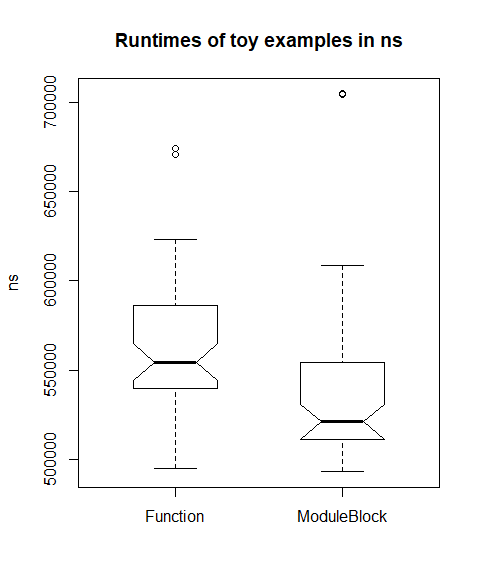
\includegraphics[scale=0.7]{figures/runtimesToyBoxplot.png}
    \caption{Benchmark boxplots for toy example}
    \label{fig:bToy}
\end{figure}

\subsection{k-means}
The second example implements a simple application of the k-means clustering algorithm.\footnote{The interested reader can find more information on the algorithm in the Journal of the Royal Statistical Society. Series C (Applied Statistics) Vol. 28, No. 1 (1979), pp. 100-108, or as a German source:  https://www-m9.ma.tum.de/material/felix-klein/clustering/Methoden/K-Means.php}
The general code setup for the module block example is shown in Listing \ref{fig:kMeans}. The module block contains all constants function declarations and calls necessary to perform a cluster calculation via the k-means algorithm. The module block then is embedded into a promise via a dynamic import. The benchmark used for the toy example is also used with the k-means algorithm. The results again show no noticeable performance overhead on the module block's part and thus recreate the findings of the toy example. Figure \ref{fig:bKMeans} summarizes the results of 50 runs and shows that in comparison to the reference runtime, function calls regularly and from module, show no better performance than the respective module block calls.

\begin{lstlisting}[caption={Module block toy example}, label={fig:kMeans}]
    // *.js module block code
    (async function() {
        var kMeans = module {
            const ...
            function() ...
            // kMeans magic
            createRandomData();
            cluster();
        };
        
        return await import(kMeans)
    })();
\end{lstlisting}

\begin{figure}[h!]
    \centering
    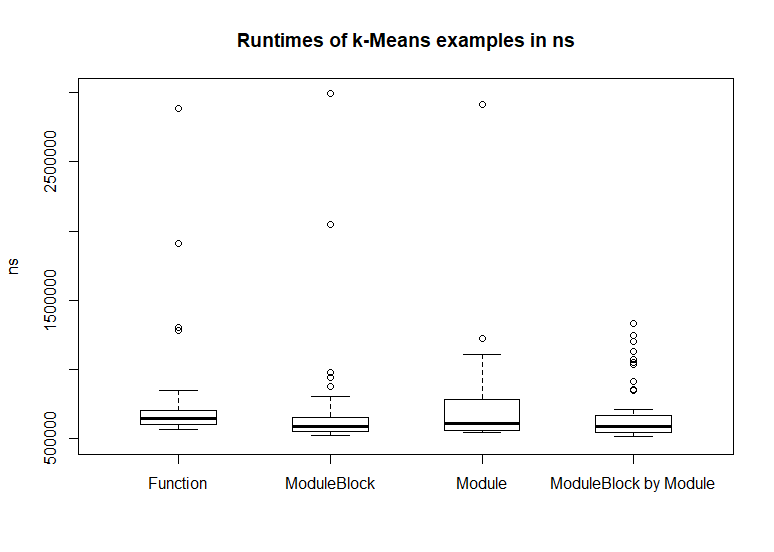
\includegraphics[scale=0.7]{figures/runtimesKMeansBoxplot.png}
    \caption{Benchmark boxplots for k-means example}
    \label{fig:bKMeans}
\end{figure}
\pagebreak
The benchmarks were conducted on a PC with Windows 10, an Intel 3700K i7 processor and 16 GB RAM. Overall it can be summarized that as the two examples show, no explicit performance loss due to module block calls can be noted. The only tendency, that can be noted, is the outliers in the module block cases. Module block code produces significantly more outliers and is thus not as reliable performance-wise as the regular function calls. 